\chapter{Numerical experiments}
\label{chap:expe}

Experiments and Python programming.

\section{Synthetic experiments}
\label{sec:synexp}

\begin{figure}[h]\centering
    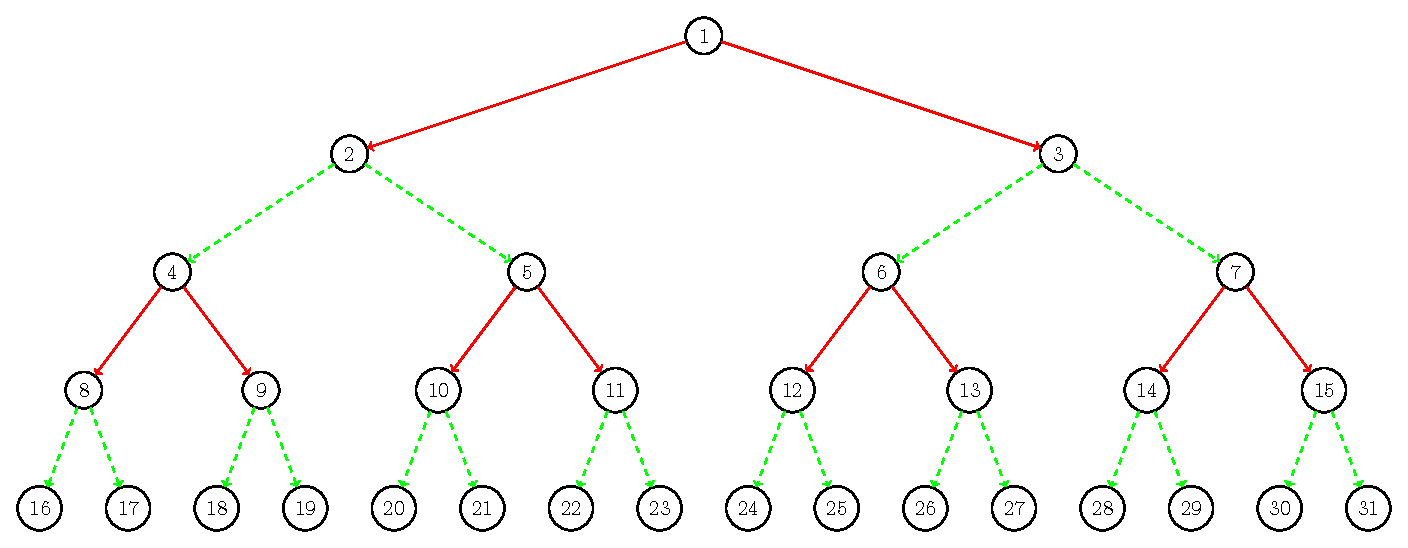
\includegraphics[width=.75\textwidth]{experiment1}
    \caption{Network structure (binary tree) for the first synthetic experiment. The active links of A(t) alternate between the solid and dashed edges, with extra noise added at each time step, over a period of 10 cycles.}
    \label{fig:exp1}
    \bigskip
\end{figure}

\begin{figure}
     \centering
     \begin{subfigure}[b]{0.4\textwidth}
         \centering
         \includegraphics[width=\textwidth]{exp1_bt20a}
         \caption{Broadcast centrality for $\alpha = 0.7 ,~\beta = 0.1$}
         \label{fig:bt1}
     \end{subfigure}
     \hspace{0.5cm}
     \begin{subfigure}[b]{0.4\textwidth}
         \centering
         \includegraphics[width=\textwidth]{exp1_bt20b}
         \caption{Broadcast centrality for $\alpha = 0.7 ,~\beta = 0.01$}
         \label{fig:bt2}
     \end{subfigure}
     
     \begin{subfigure}[b]{0.4\textwidth}
         \centering
         \includegraphics[width=\textwidth]{exp1_bt20c}
         \caption{Broadcast centrality for $\alpha = 0.1 ,~\beta = 0.1$}
         \label{fig:bt3}
     \end{subfigure}
     \hspace{0.5cm}
     \begin{subfigure}[b]{0.4\textwidth}
         \centering
         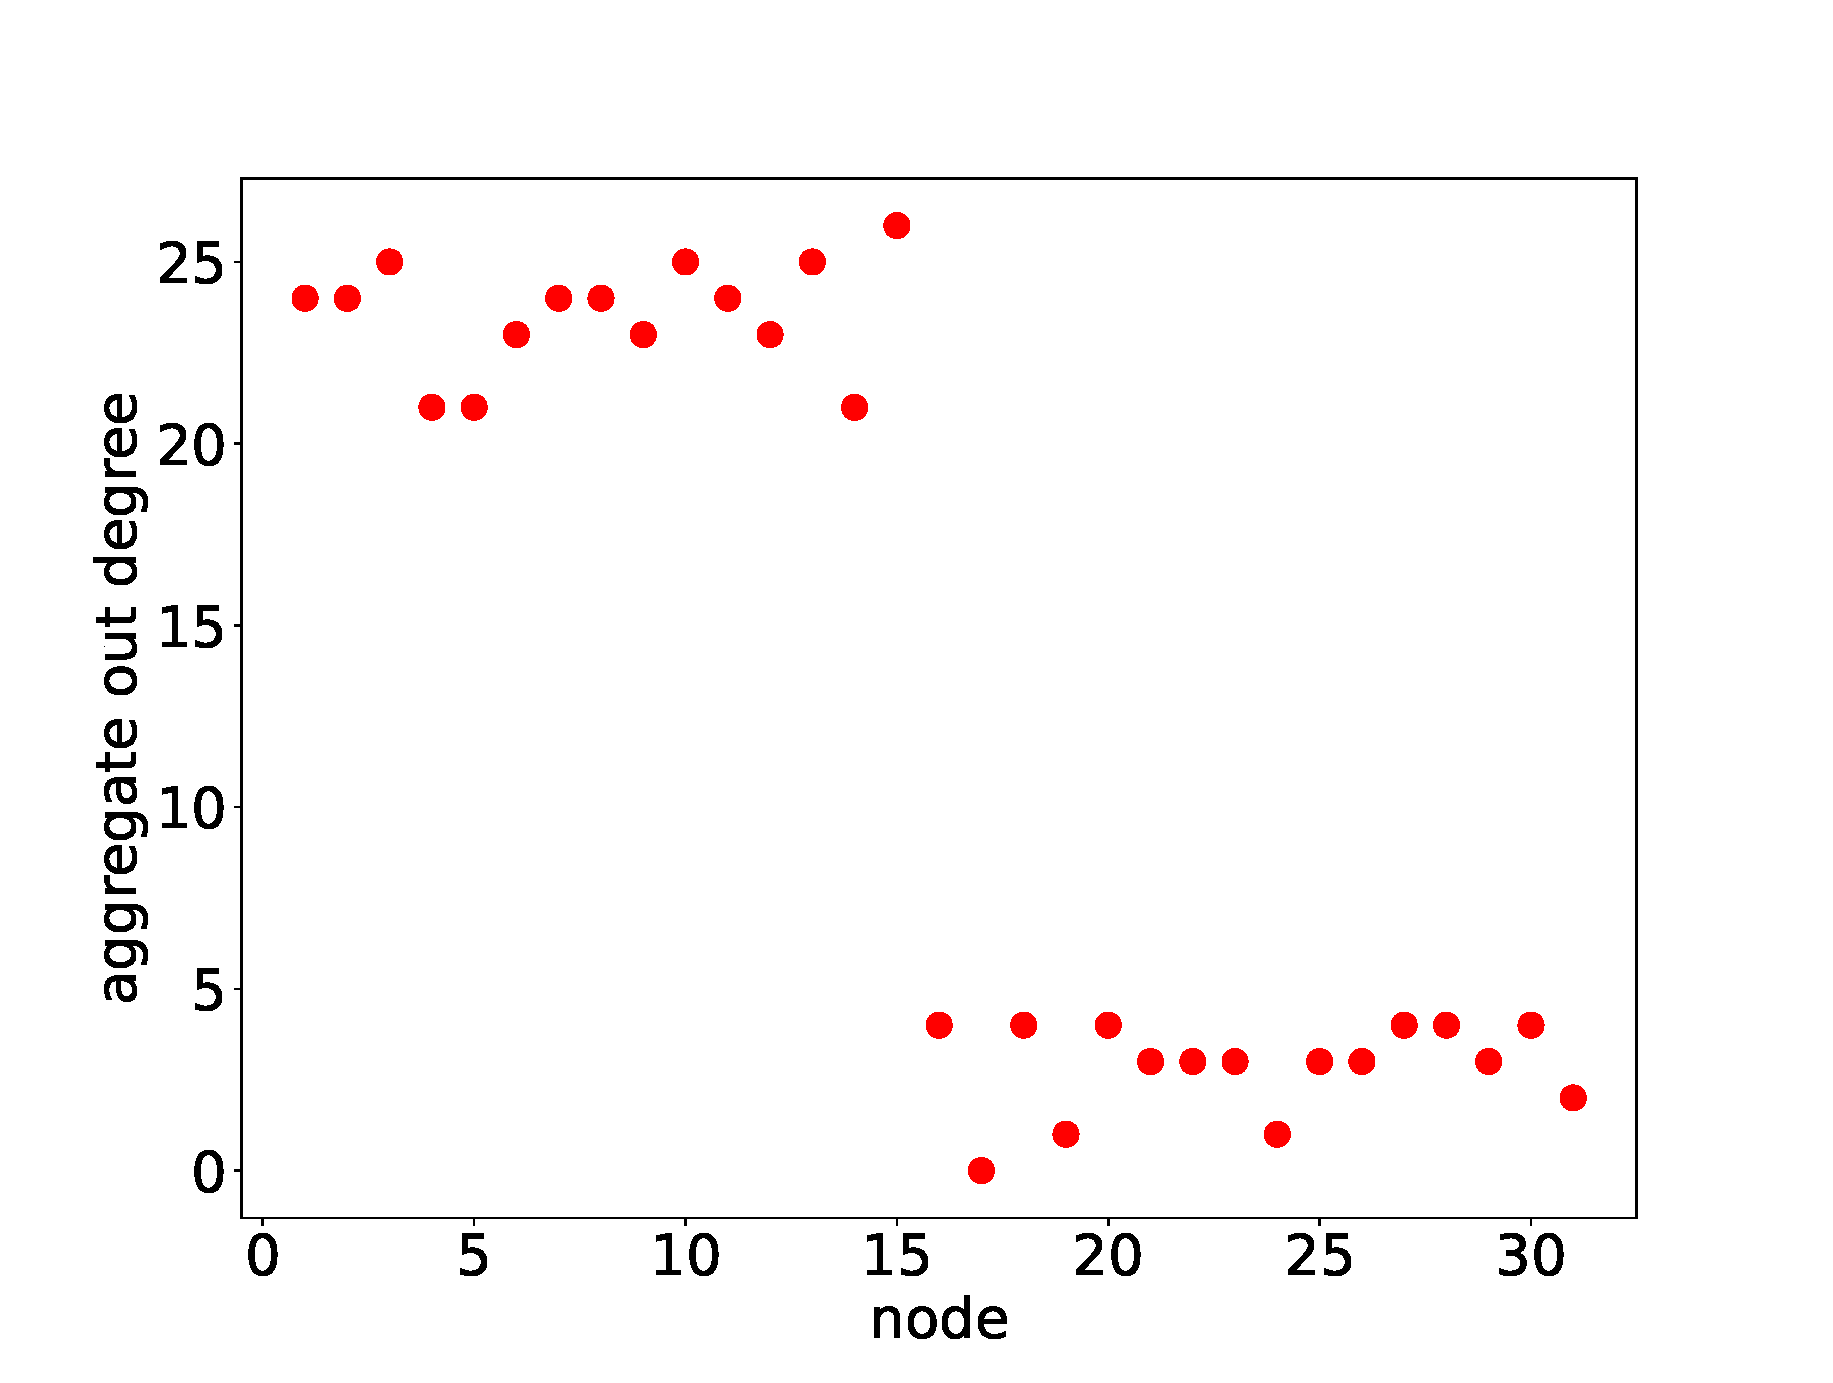
\includegraphics[width=\textwidth]{exp1_agg_out_degree}
         \caption{Aggregate out degree for each node}
         \label{fig:bt4}
     \end{subfigure}
        \caption{Results from the dynamic network in figure \ref{fig:exp1}.}
        \label{fig:fourbt}
\end{figure}

\begin{figure}[h]\centering
    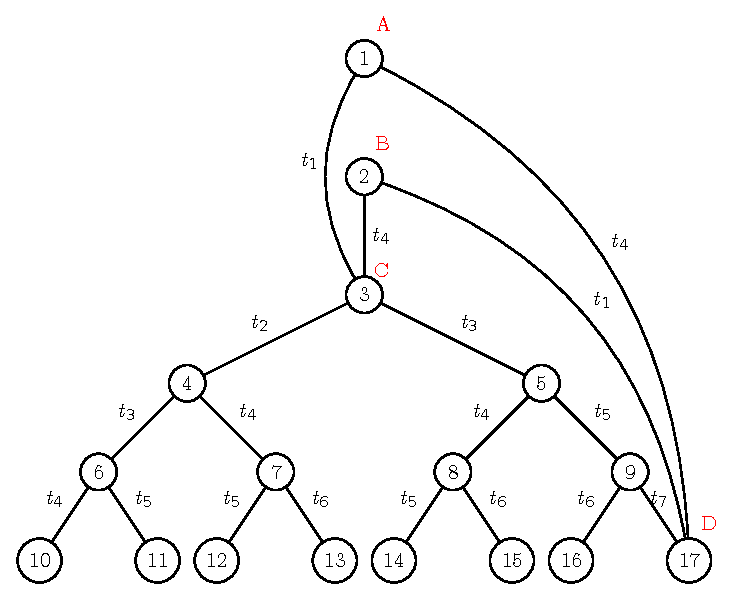
\includegraphics[width=.65\textwidth]{experiment2}
    \caption{Network structure for the second synthetic experiment. Links of A(t) are active over non-overlapping time intervals such that $t_i\coloneqq[(i − 1)\tau , (i − 1 + 0.9)\tau )$, for $i=0, 1, \dots , 7$, and $\tau =0.1$, repeated periodically over five cycles.}
    \label{fig:exp2}
    \bigskip
\end{figure}

\begin{figure}
     \centering
     \begin{subfigure}[b]{0.49\textwidth}
         \centering
         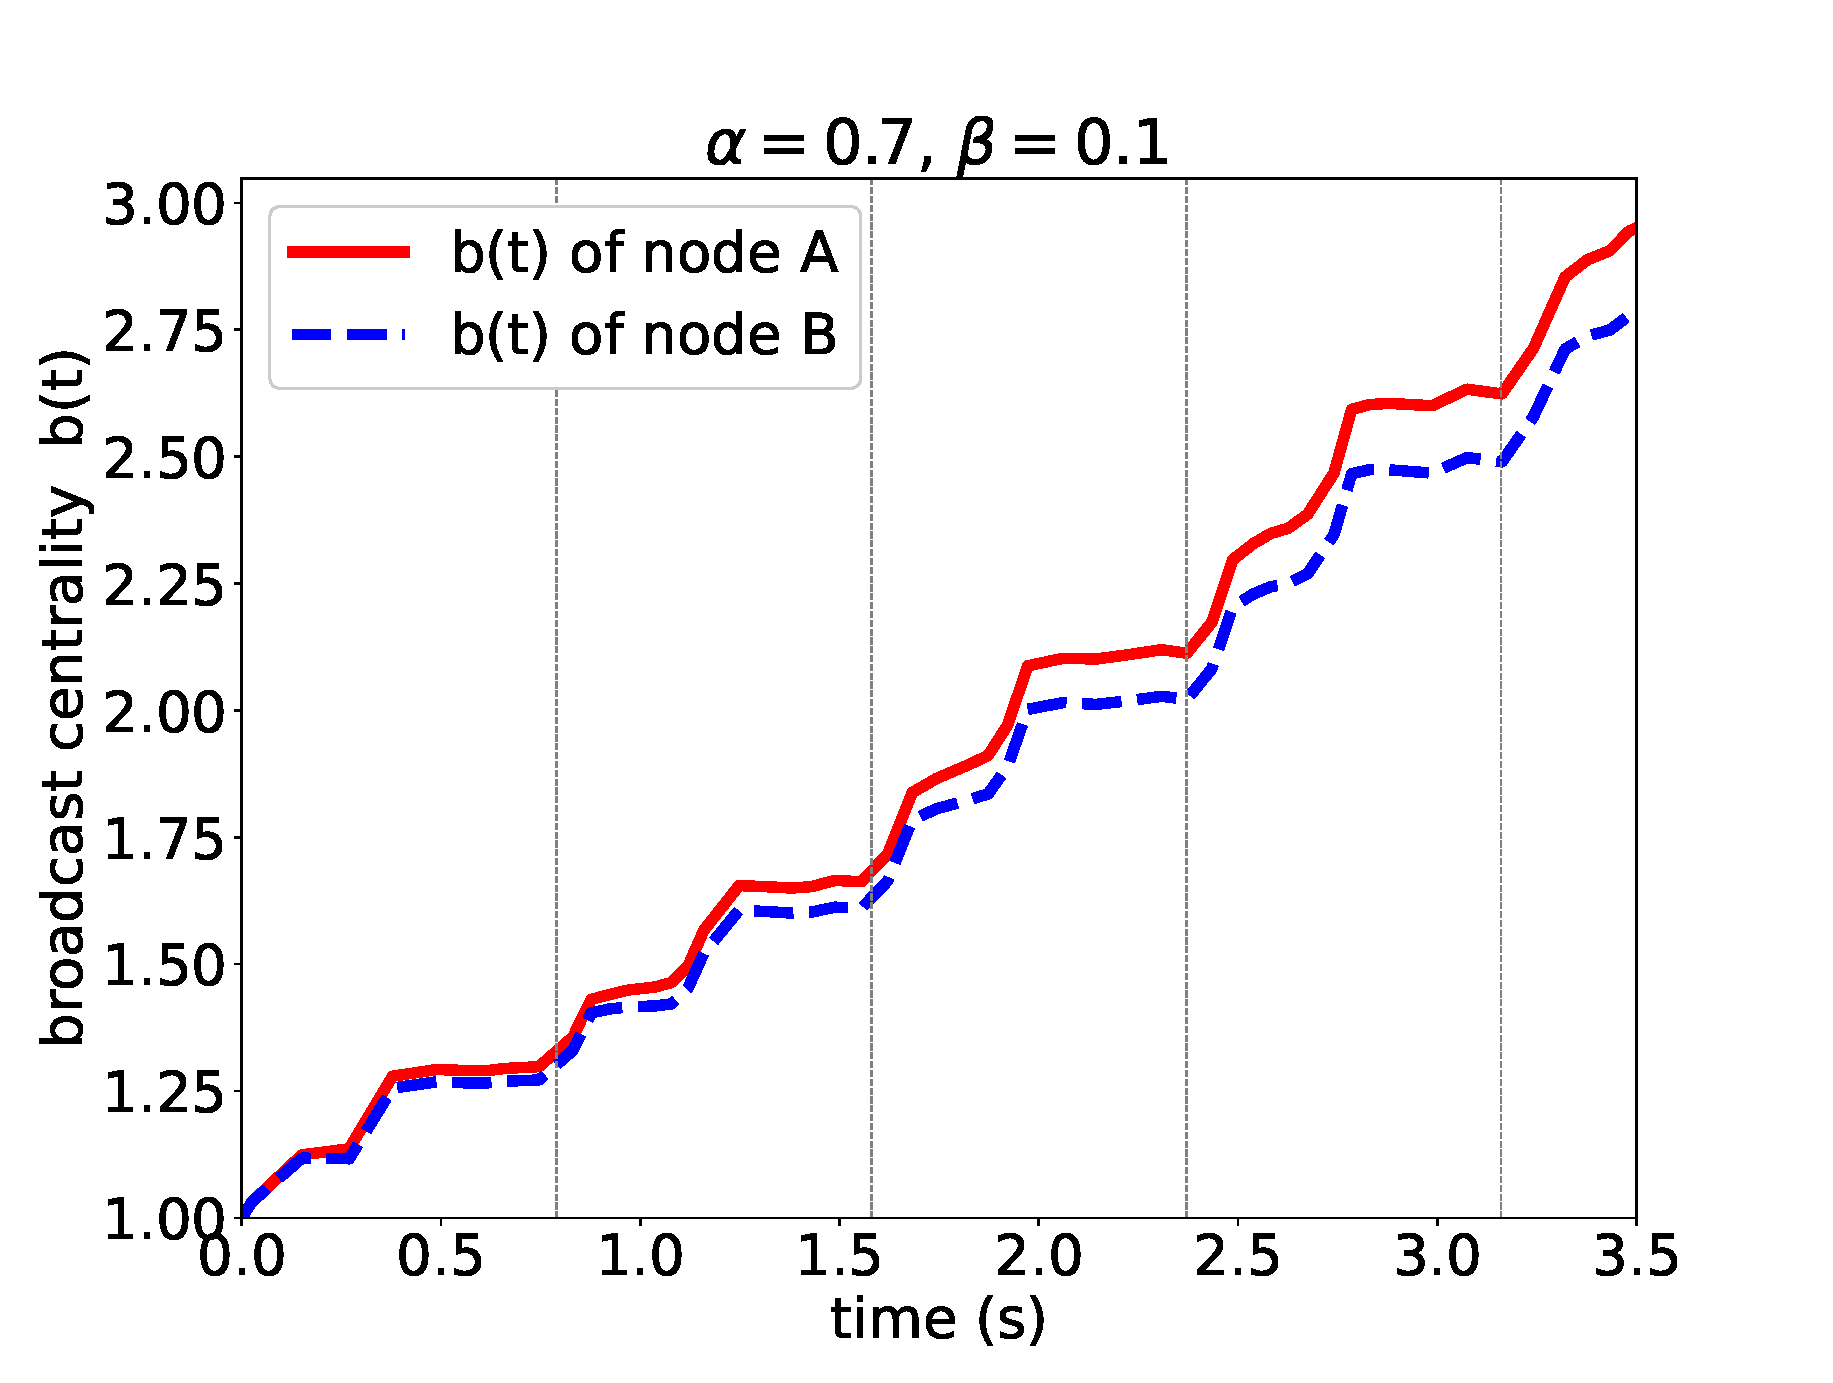
\includegraphics[width=\textwidth]{exp2b_btA_vs_btB}
         \caption{broadcast for $\alpha = 0.7 ,~\beta = 0.1$}
         \label{fig:bt5}
     \end{subfigure}
     \hfill
     \begin{subfigure}[b]{0.49\textwidth}
         \centering
         \includegraphics[width=\textwidth]{exp2a_btA_vs_btB}
         \caption{broadcast for $\alpha = 0.9 ,~\beta = 0.1$}
         \label{fig:bt6}
     \end{subfigure}
     \caption{Dynamic broadcast centrality over time for node A (solid) and node B (dashed) in the network of figure \ref{fig:exp2}.}
     \label{fig:twobt}
\end{figure}


\section{Voice call experiment}
\label{sec:voicecall}

